\documentclass[table]{beamer}
\mode<presentation>
\usetheme{Berlin}
\usecolortheme{beaver}
\usepackage{listings}
\usepackage{multirow}
\usepackage{xcolor}

%%%
% LISTINGS SETTING
\lstset{ %
  backgroundcolor=\color{yellow},   % choose the background color; you must add \usepackage{color} or \usepackage{xcolor}
  basicstyle=\tiny\ttfamily,        % the size of the fonts that are used for the code
  breakatwhitespace=false,         % sets if automatic breaks should only happen at whitespace
  breaklines=true,                 % sets automatic line breaking
  captionpos=b,                    % sets the caption-position to bottom
  commentstyle=\color{red},    % comment style
  deletekeywords={...},            % if you want to delete keywords from the given language
  escapeinside={\%*}{*)},          % if you want to add LaTeX within your code
  extendedchars=true,              % lets you use non-ASCII characters; for 8-bits encodings only, does not work with UTF-8
  frame=single,                    % adds a frame around the code
  keepspaces=true,                 % keeps spaces in text, useful for keeping indentation of code (possibly needs columns=flexible)
  keywordstyle=\color{blue},       % keyword style
%  language=Octave,                 % the language of the code
  morekeywords={*,...},            % if you want to add more keywords to the set
  numbers=left,                    % where to put the line-numbers; possible values are (none, left, right)
  numbersep=5pt,                   % how far the line-numbers are from the code
  numberstyle=\tiny\color{gray}, % the style that is used for the line-numbers
  rulecolor=\color{black},         % if not set, the frame-color may be changed on line-breaks within not-black text (e.g. comments (green here))
  showspaces=false,                % show spaces everywhere adding particular underscores; it overrides 'showstringspaces'
  showstringspaces=false,          % underline spaces within strings only
  showtabs=false,                  % show tabs within strings adding particular underscores
  stepnumber=1,                    % the step between two line-numbers. If it's 1, each line will be numbered
  stringstyle=\color{violet},     % string literal style
  tabsize=4,                       % sets default tabsize to 2 spaces
  title=\lstname                   % show the filename of files included with \lstinputlisting; also try caption instead of title
}

%%%
% TITLE PREAMBLE
\title[Intro to Bioinformatics] % (optional, only for long titles)
{Introduction to Bioinformatics}
\subtitle{Part 0: So You Want To Be a Computational Biologist?}
\author[Pritchard, Cock] % (optional, for multiple authors)
{Leighton~Pritchard \and Peter~Cock}
\institute[The James Hutton Institute] % (optional)
{
  Information and Computational Sciences\\
  The James Hutton Institute
}
\date[May 2014] % (optional)
{Bioinformatics Training, 29$^{th}$, 30$^{th}$ May 2014}
\subject{Bioinformatics}

%%%
% TOC
% Show table of contents, with current section highlighted,
% at the start of each section
\AtBeginSection[]
{
  \begin{frame}
    \frametitle{Table of Contents}
    \tableofcontents[currentsection]
  \end{frame}
}


%%%
% START DOCUMENT
\begin{document}

  \frame[plain]{\titlepage}
  
  \begin{frame}
    \frametitle{Bertrand Russell}
    \begin{center}
      
\includegraphics[width=\textwidth]{images/bertrand}
    \end{center}
  \end{frame}
    
 %%%
 % SECTION: Introduction
  \section{Introduction}
  \subsection{So You Want To Be a Computational Biologist?}
  \begin{frame}
    \frametitle{What is this ``bioinformatics'' thing, anyway?}
    \begin{itemize}
      \item Bioinformatics: biology using computational and mathematical tools
      \item A discipline within biology
      \begin{itemize}
        \item Loman \& Watson (2013) ``So you want to be a computational biologist?''
        \url{http://dx.doi.org/10.1038/nbt.2740}
        \item Welch \textit{et al.} (2014) ``Bioinformatics Curriculum Guidelines: Toward a Definition of Core Competencies''
        \url{http://dx.doi.org/10.1371/journal.pcbi.1003496}
        % http://bit.ly/1fS4iDJ links to http://biomickwatson.wordpress.com/2014/03/10/the-only-core-competency-youre-ever-going-to-need/}
        \item Watson (2014) ``The only core competency you need'' \url{http://bit.ly/1fS4iDJ} (blog)
      \end{itemize}
    \end{itemize}
  \end{frame}

  \begin{frame}
    \frametitle{Some uncomfortable truths}
    \begin{itemize}
      \item This one-day course will not make you a bioinformatician
      \item The best way to learn is to do (``I don't know how to do this yet, but I will find out.'')
      % http://bit.ly/Rq0D61 links to http://biomickwatson.wordpress.com/2013/08/06/bioinformatics-is-not-something-you-are-taught-its-a-way-of-life/
      \begin{itemize}
        \item \url{http://bit.ly/Rq0D61} (``Bioinformatics is a way of life'')
      \end{itemize}
      \item Most bioinformatics is problem-solving
      \item We will introduce some useful tools and concepts
    \end{itemize}
  \end{frame}

  \begin{frame}
    \frametitle{What it takes to be a bioinformatician}
    \begin{columns}[t]
      \begin{column}{5cm}
        \begin{itemize}
          \item Patience (problem-solving)
          \item Suspicion (statistics)
          \item Biological knowledge
          \item Social skills (no-one knows everything: ask!)
	      \item Lots of practice          
	    \end{itemize}
	  \end{column}
	  \begin{column}{5cm}
	    \begin{itemize}
	      \item Self-confidence (challenge results and dogma)
	      \item Core domain skills: biology, computer science, statistics
	      \item Deliver results (qualified, honest)
	    \end{itemize}
	  \end{column}
	\end{columns}
	\begin{itemize}
	  % http://bit.ly/1jDuQsO link goes to http://biomickwatson.wordpress.com/2013/03/18/the-alternative-what-it-takes-to-be-a-bioinformatician/
	  \item Watson (2014) ``What it takes to be a bioinformatician'' \url{http://bit.ly/1jDuQsO} (blog)
	  %\item \url{http://science.slashdot.org/comments.pl?sid=3161217&cid=41542125}
	\end{itemize}
  \end{frame}


   \begin{frame}
     \frametitle{More general advice?}
     \begin{itemize}
	   \item Ask us (we do this a lot)
	   \item BioStars (\url{https://www.biostars.org})
	   \item SeqAnswers (\url{http://seqanswers.com/})
	   \item \textit{PLoS Comp Biol} collections (\url{http://www.ploscollections.org/static/pcbiCollections})
	\end{itemize}
	
\includegraphics[width=.2\textwidth]{images/gibas_book}
	
\includegraphics[width=.2\textwidth]{images/buffalo_book}
	
\includegraphics[width=.18\textwidth]{images/bassi_book}
	
\includegraphics[width=.2\textwidth]{images/korf_book}
	
\includegraphics[width=.2\textwidth]{images/model_book}
   \end{frame}

 %%%
 % SECTION: Recording your work
   \section{Recording Your Work}
   
   % SUBSECTION: justification
   \subsection{Why and How?}
   \begin{frame}
     \frametitle{Why Do It?}
     \begin{itemize}
	   \item Doing bioinformatics is doing science: keep a lab book!
	   \item You \emph{will not} remember multiple files, analysis details, etc. in a week/month/six months/a year/three years
	   \begin{itemize}
	     \item Noble (2009) \url{http://dx.doi.org/10.1371/journal.pcbi.1000424}
	     \item Baggerly \& Coombes (2009) \url{http://arxiv.org/pdf/1010.1092.pdf}
	   \end{itemize}
	\end{itemize}
	
\includegraphics[width=.6\textwidth]{images/noble_2009_head}
   \end{frame}
   
   \begin{frame}
     \frametitle{How To Do It? I}
     \begin{itemize}
	   \item There is no one correct way, but$\ldots$
	   \item Think about data/docs/project structure \textit{before} you start
    \end{itemize}
    \begin{center}
      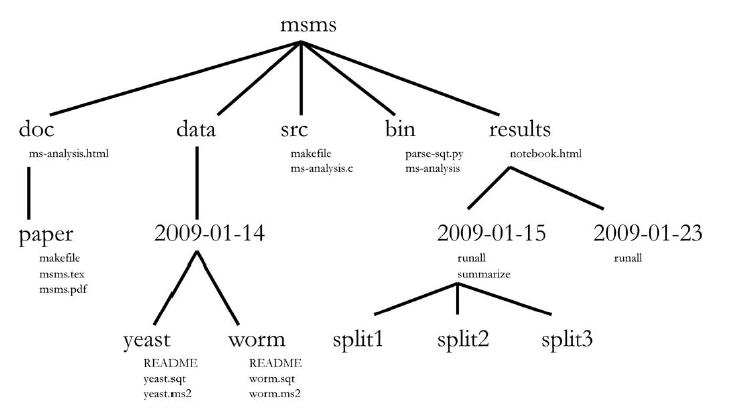
\includegraphics[width=.5\textwidth]{images/project_structure}
      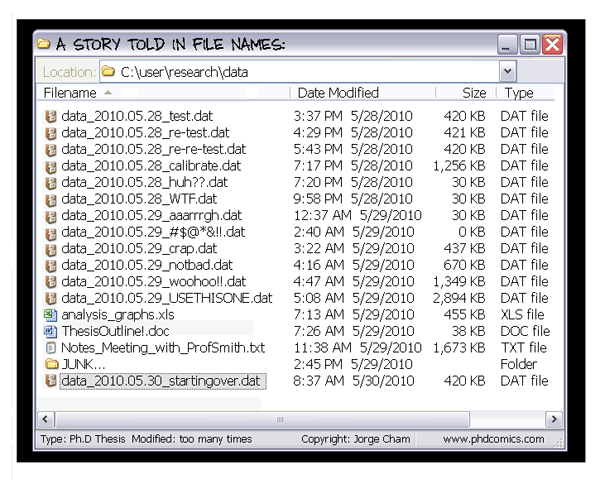
\includegraphics[width=.5\textwidth]{images/phd052810s}
    \end{center}
   \end{frame}

   \begin{frame}
     \frametitle{How To Do It? II}
     \begin{itemize}
	   \item Use plain text where possible
	   \item Use version control
	   \item Keep backups
	   \item Different tools suit different purposes: code \textit{vs.} data \textit{vs.} analysis \textit{vs.} $\ldots$
	   \item Find a way that works \emph{for you}.
	\end{itemize}
   \end{frame}

   \begin{frame}
     \frametitle{How To Do It? III}
     \begin{itemize}
	   \item Reproducibility is key!
	   \item Scripts and pipelines are better for this than notes of what you did
	   \begin{itemize}
	     \item Also better for version control, and reuse
	   \end{itemize}
	   \item Avoid unnecessary duplication
	   \begin{itemize}
	     \item Someone else may have solved your problem
	     \item One (backed up) read-only copy of raw data, keep analyses separate
	   \end{itemize}
	\end{itemize}
   \end{frame}
   
   
   % SUBSECTION: useful tools
   \subsection{Useful Tools for Recording Your Work}
   \begin{frame}
     \frametitle{Plain Text Files}
     \begin{itemize}
       \item \texttt{README.txt}/\texttt{README.md} in each directory/folder
       \item Plain text is always human-readable
       \begin{itemize}
         \item Markdown (\url{https://daringfireball.net/projects/markdown/basics})
         \item RST (\url{http://docutils.sourceforge.net/docs/ref/rst/restructuredtext.html})
       \end{itemize}
     \end{itemize}
     \begin{center}
       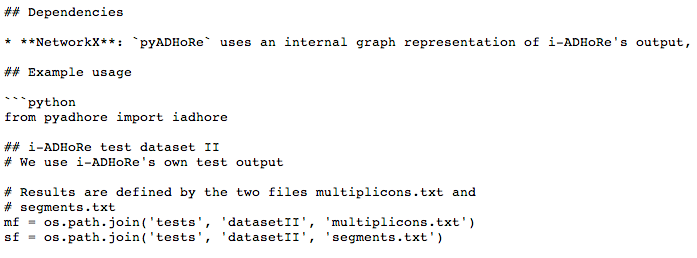
\includegraphics[width=.4\textwidth]{images/markdown_before}
       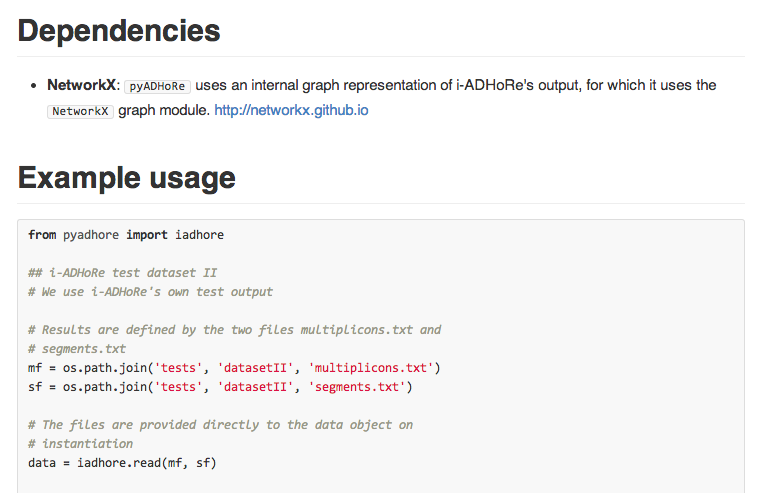
\includegraphics[width=.4\textwidth]{images/markdown_after}
     \end{center}
   \end{frame}
   
   \begin{frame}
     \frametitle{Galaxy workflows}
     \begin{itemize}
       \item Use through browser, graphical interface
       \item Reproducible, shareable, documented, reusable analyses
       \item Wraps standard bioinformatics tools
       \item Local instance (\url{http://ppserver/galaxy}) uses JHI cluster       
     \end{itemize}
     \begin{center}
       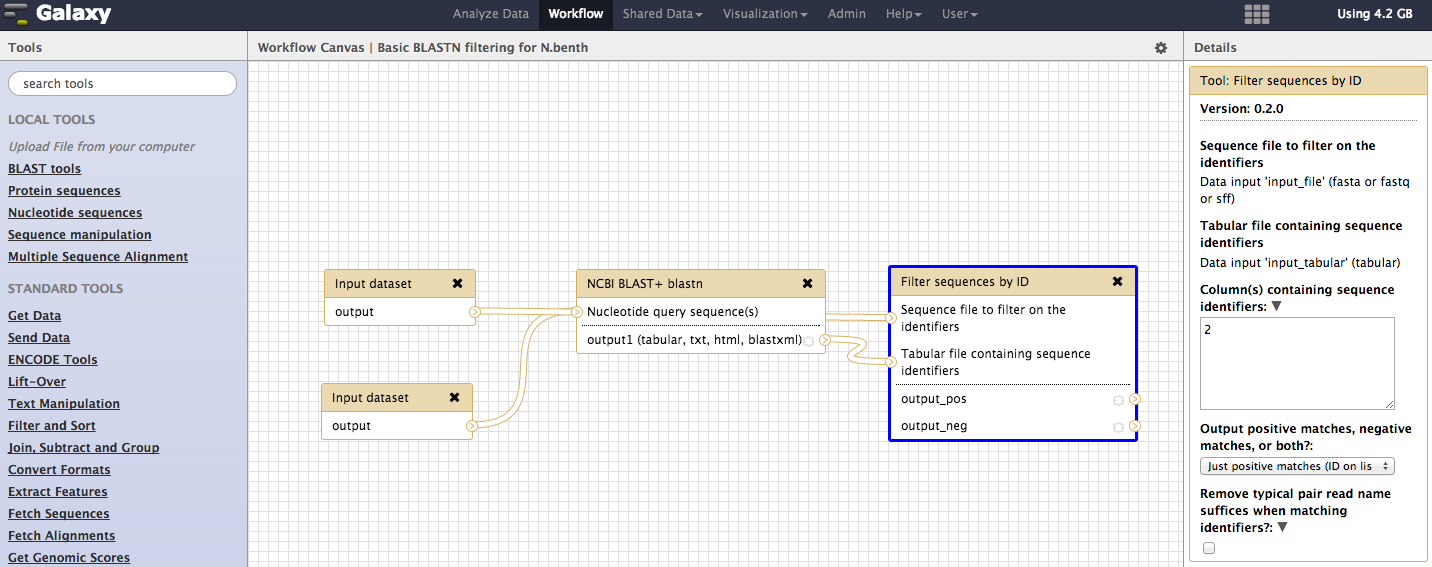
\includegraphics[width=.75\textwidth]{images/galaxy_screenshot}
     \end{center}
   \end{frame}      
   
   \begin{frame}
     \frametitle{\texttt{script}}
     \begin{itemize}
       \item Writes your terminal activity to a plain text file
       \item Saves effort copy/pasting and typing commands into a lab book, as you go
       \item Easy to use with other tools 
       \item use \texttt{man script} at your terminal to find out more
     \end{itemize}
   \end{frame}   
   
   \begin{frame}
     \frametitle{MediaWiki}
     \begin{itemize}
       \item Useful for shared projects/data
       \item Automatic version control and attribution
       \item Many local instances at JHI (ask around)
     \end{itemize}
     \begin{center}
       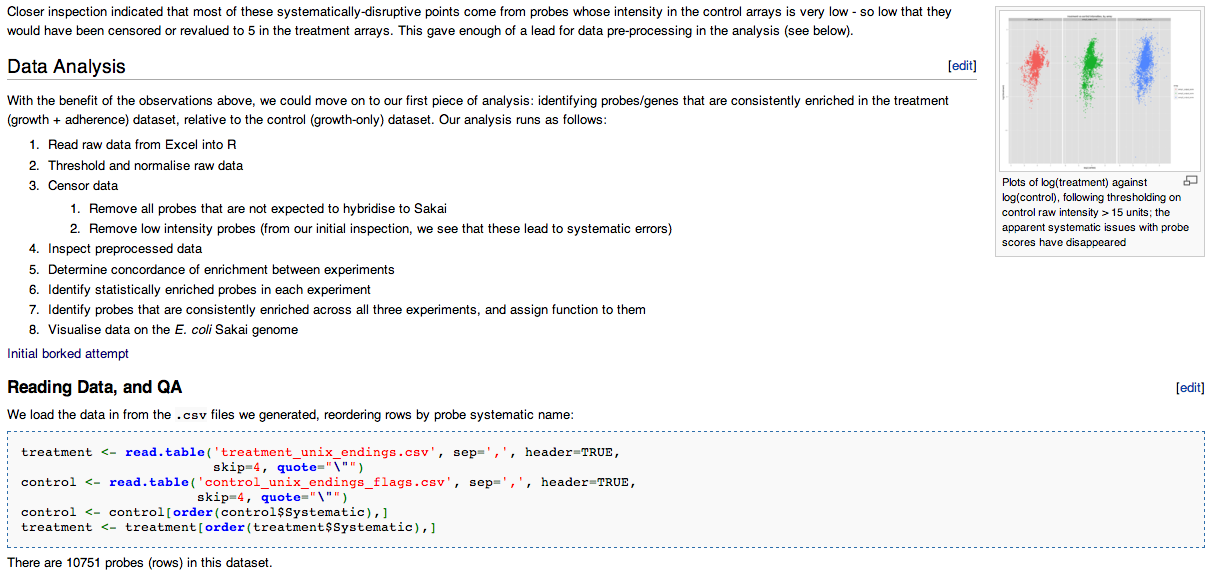
\includegraphics[width=.4\textwidth]{images/mediawiki_after}
       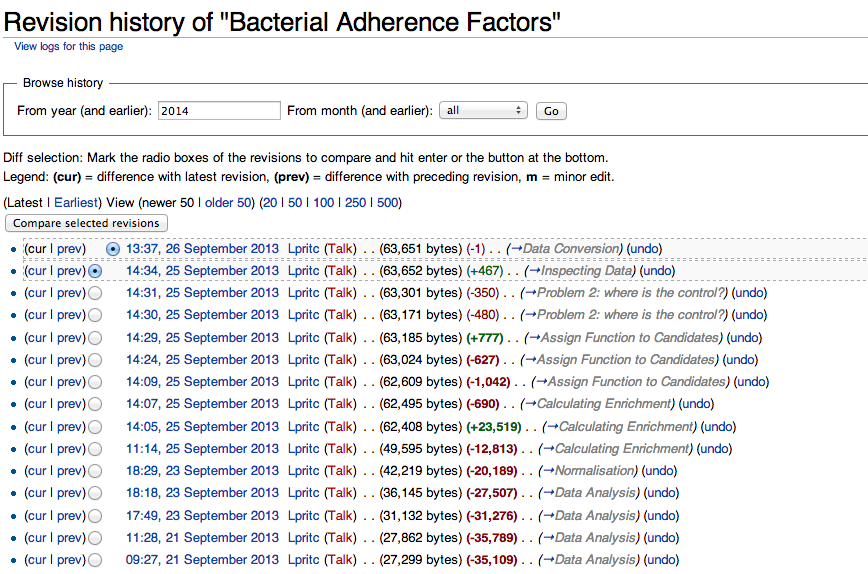
\includegraphics[width=.4\textwidth]{images/mediawiki_version_control}     
     \end{center}
   \end{frame}
   
   \begin{frame}
     \frametitle{A language notebook}
     \begin{itemize}
       \item e.g. \texttt{iPython Notebook}, \texttt{Mathematica}, \texttt{MatLab} cells
       \item Integrates live code and analysis with lab-book
     \end{itemize}
     \begin{center}
       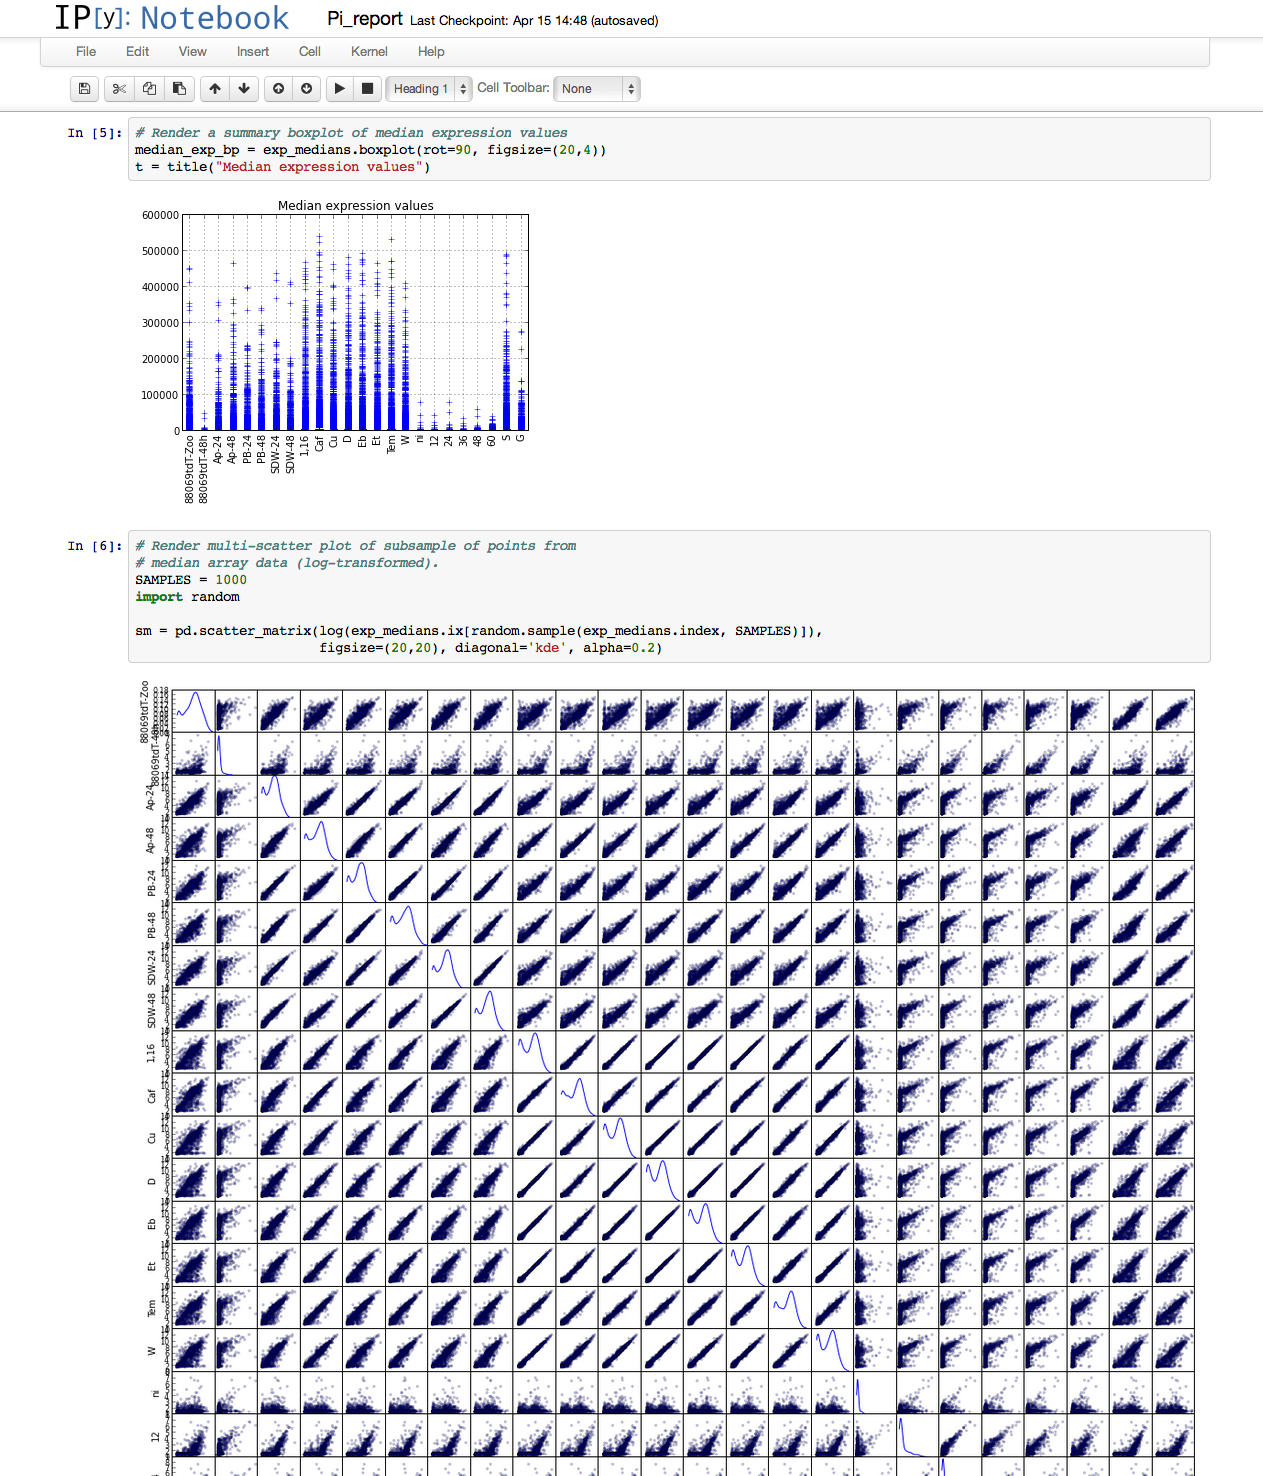
\includegraphics[width=.35\textwidth]{images/ipython_notebook}     
     \end{center}
   \end{frame}

   \begin{frame}
     \frametitle{\LaTeX}
     \begin{itemize}
       \item Powerful, versatile typesetting system
       \item Similar to markup/markdown
       \item Pros: great for mathematical/computing work, writing a thesis
       \item Cons: not easy to pick up
     \end{itemize}
     \begin{center}
        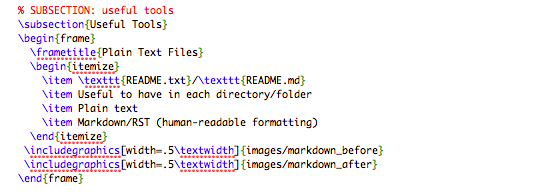
\includegraphics[width=.35\textwidth]{images/latex_before}
        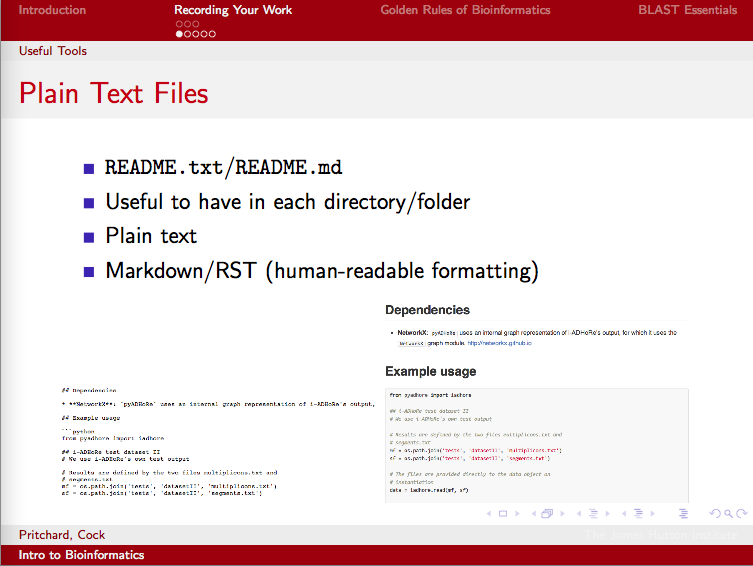
\includegraphics[width=.35\textwidth]{images/latex_after}     
     \end{center}
   \end{frame}

% etc
\end{document}